\section{The dot product}
\label{sec:dot-product}

\begin{outcome}
  \begin{enumerate}
  \item Compute the dot product of vectors geometrically and
    algebraically.
  \item Use properties of the dot product, including the
    Cauchy-Schwarz inequality and the triangle inequality, to prove
    further equalities and inequalities.
  \item Determine whether two vectors are orthogonal.
  \item Compute the scalar and vector projection of one vector onto
    another.
  \item Decompose a vector into orthogonal components.
  \end{enumerate}
\end{outcome}

There are two ways of multiplying vectors that are useful in
applications. The first of these is called the \textbf{dot product},
and the second is called the \textbf{cross product}. We will consider
the dot product here, and the cross product in the next section.

% ----------------------------------------------------------------------
\subsection{Definition and properties}

When we take the dot product of two vectors, the result is a
scalar. For this reason, the dot product is also called the
\textbf{scalar product}. Sometimes it is also called the \textbf{inner
  product}. The definition is as follows\index{dot product}%
\index{vector!dot product}%
\index{scalar product|see{dot product}}%
\index{inner product|seealso{dot product}}.

\begin{definition}{Dot product}{dot-product}
  Let $\vect{u}=\begin{mymatrix}{c}
    u_1 \\
    u_2 \\
    \vdots \\
    u_n
  \end{mymatrix}$, $\vect{v}= \begin{mymatrix}{c}
    v_1 \\
    v_2 \\
    \vdots \\
    v_n
  \end{mymatrix}$ be two vectors in $\R^{n}$. We
  define their \textbf{dot product} as
  \begin{equation*}
    \vect{u}\dotprod \vect{v} = u_1v_1+u_2v_2+\ldots+u_nv_n.
  \end{equation*}
\end{definition}

\begin{example}{Compute a dot product}{dot-product}
  Find $\vect{u} \dotprod \vect{v}$ for $\vect{u}=\mat{1,2,0,-1}^T$
  and $\vect{v}=\mat{0,1,2,3}^T$.
\end{example}

\begin{solution}
  We have
  \begin{eqnarray*}
    \vect{u} \dotprod \vect{v}
    &=&
        (1)(0) + (2)(1) + (0)(2) + (-1)(3) \\
    &=&
        0 + 2 + 0 + -3 \\
    &=&
        -1.
  \end{eqnarray*}
\end{solution}

The dot product satisfies a number of important properties.

\begin{theorem}{Properties of the dot product}{properties-dot-product}
  \index{dot product!properties}%
  \index{properties of dot product}%
  \index{vector!dot product!properties}%
  \index{vector!properties of dot product}%
  The dot product satisfies the following properties, where
  $\vect{u},\vect{v},\vect{w}$ are vectors and $k,\ell$ are
  scalars.
  \begin{itemize}
  \item $\vect{u}\dotprod\vect{v}=\vect{v}\dotprod\vect{u}$.
  \item $\vect{u}\dotprod\vect{u}\geq 0$, and $\vect{u}\dotprod\vect{u}=0$ if and only if $\vect{u}=\vect{0}$.
  \item $(k\vect{u}+\ell\vect{v})\dotprod\vect{w}=k(\vect{u}\dotprod\vect{w})+\ell(\vect{v}\dotprod\vect{w})$.
  \item $\vect{u}\dotprod(k\vect{v}+\ell\vect{w})
    =k(\vect{u}\dotprod \vect{v})+\ell(\vect{u}\dotprod\vect{w})$.
  \item $\vect{u}\dotprod\vect{u}=\norm{\vect{u}}^{2}$.
  \end{itemize}
\end{theorem}

The proof is left as an exercise. Note that, by the last part of the
theorem, we can also use the dot product to find the length of a
vector.

\begin{example}{Length of a vector}{dot-product-length}
  Use a dot product to find $\norm{\vect{u}}$, where
  \begin{equation*}
    \vect{u}
    =
    \begin{mymatrix}{r}
      2 \\
      1 \\
      4 \\
      2
    \end{mymatrix}.
  \end{equation*}
\end{example}

\begin{solution}
  By the last part of Theorem~\ref{thm:properties-dot-product}, we have
  $\norm{\vect{u}} = \sqrt {\vect{u} \dotprod \vect{u}}$. We have
  $\vect{u} \dotprod \vect{u} = 2^2+1^2+4^2+2^2 = 25$, and therefore
  $\norm{\vect{u}} = \sqrt{\vect{u} \dotprod \vect{u}} = \sqrt{25} = 5$.
\end{solution}

% ----------------------------------------------------------------------
\subsection{The Cauchy-Schwarz and triangle inequalities}

The \textbf{Cauchy-Schwarz inequality}%
\index{Cauchy-Schwarz inequality!for dot product} is a fundamental
inequality satisfied by the dot product.  It is given in the following
theorem.

\begin{theorem}{Cauchy-Schwarz inequality}{cauchy-schwarz-inequality}
  The dot product satisfies the inequality
  \begin{equation}\label{cauchy}
    \abs{\vect{u}\dotprod \vect{v}}\leq \norm{\vect{u}} \norm{\vect{v}}
  \end{equation}
  Furthermore equality is obtained if and only if one of $\vect{u}$ or $\vect{v}$ is a scalar multiple of the other.
\end{theorem}

\begin{proof}
  First note that if $\vect{u}=\vect{0}$, then both sides of
  \eqref{cauchy} are equal to zero, and so the inequality holds in
  this case. Therefore, we will assume in what follows that
  $\vect{u}\neq \vect{0}$.  Define a function of $t\in \R$ by
  \begin{equation*}
    f(t) =(t\vect{u}+\vect{v}) \dotprod (t\vect{u}+ \vect{v}).
  \end{equation*}
  Then by Theorem~\ref{thm:properties-dot-product}, $f(t) \geq 0$
  for all $t\in \R$.  Also from
  Theorem~\ref{thm:properties-dot-product}, we have
  \begin{eqnarray*}
    f(t) &=&t\vect{u}\dotprod (t\vect{u}+\vect{v}) +
             \vect{v}\dotprod (t\vect{u}+\vect{v}) \\
         &=&t^2\vect{u}\dotprod \vect{u}+t(\vect{u}\dotprod \vect{v}) + t \vect{v}\dotprod \vect{u}+
             \vect{v}\dotprod \vect{v} \\
         &=&t^2\norm{\vect{u}}^{2}+2t(\vect{u}\dotprod \vect{v}) +\norm{
             \vect{v}} ^{2}.
  \end{eqnarray*}
  This means the graph of $y=f(t)$ is a parabola which opens upwards
  and is never negative. It follows that this function has at most one
  root. From the quadratic formula, we know that a quadratic function
  $at^2+bt+c$ has one or zero roots if and only if $b^2-4ac\leq
  0$. Applying this reasoning to the function $f(t)$, we obtain
  \begin{equation*}
    (2(\vect{u}\dotprod \vect{v})) ^{2}-4\norm{\vect{u}
    } ^{2}\norm{\vect{v}} ^{2}<0,
  \end{equation*}
  which is equivalent to
  $\abs{\vect{u}\dotprod \vect{v} }<\norm{\vect{u}} \norm{\vect{v}}$.
\end{proof}

An important consequence of the Cauchy-Schwarz inequality is the
so-called \textbf{triangle inequality}%
\index{triangle inequality!of vectors}, which states that the length
of one side of a triangle is less than or equal the sum of the lengths
of the two other sides.

\begin{theorem}{Triangle inequality}{triangle-inequality-dot-product}
  For\/ $\vect{u},\vect{v}\in \R^{n}$, we have
  \begin{equation}\label{triangle-ineq-1}
    \norm{\vect{u}+\vect{v}} \leq \norm{\vect{u}} +\norm{\vect{v}}.
  \end{equation}

  \begin{center}
    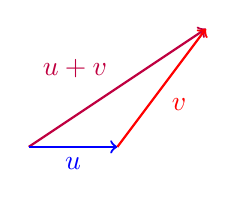
\begin{tikzpicture}[scale=1.5]
      \draw[->, thick, purple](0,0) -- node[above left]{$\vect{u}+\vect{v}$}(1.5,1);
      \draw[->, thick, blue](0,0) -- node[below]{$\vect{u}$} (0.75,0);
      \draw[->, thick, red](0.75,0) -- node[below right]{$\vect{v}$} (1.5,1);
    \end{tikzpicture}
  \end{center}
\end{theorem}

\begin{proof}
  By properties of the dot product and the Cauchy-Schwarz inequality,
  we have
  \begin{eqnarray*}
    \norm{\vect{u}+\vect{v}}^{2}
    &=& (\vect{u}+\vect{v})\dotprod(\vect{u}+\vect{v}) \\
    & =&(\vect{u}\dotprod\vect{u})+(\vect{u}\dotprod\vect{v})+(\vect{v}\dotprod\vect{u})+(\vect{v}\dotprod\vect{v}) \\
    &=&\norm{\vect{u}}^{2}+2(\vect{u}\dotprod\vect{v})+\norm{\vect{v}}^{2} \\
    &\leq& \norm{\vect{u}}^{2}+2\abs{\vect{u}\dotprod\vect{v}}+\norm{\vect{v}}^{2} \\
    &\leq& \norm{\vect{u}}^{2}+2\norm{\vect{u}}\norm{\vect{v}}+\norm{\vect{v}}^{2} =(\norm{\vect{u}}+\norm{\vect{v}})^{2}.
  \end{eqnarray*}
  Therefore,
  \begin{equation*}
    \norm{\vect{u}+\vect{v}}^{2}\leq(\norm{\vect{u}}+\norm{\vect{v}})^{2}.
  \end{equation*}
  Taking square roots of both sides, we obtain \eqref{triangle-ineq-1}.
\end{proof}

\begin{example}{Triangle inequality}{triangle-inequality}
  Use the triangle inequality to show
  \begin{equation*}
    \norm{\vect{u}} -\norm{\vect{v}} \leq \norm{\vect{u}-\vect{v}}
  \end{equation*}
  holds for all vectors $\vect{u},\vect{v}\in\R^n$.
\end{example}

\begin{solution}
  We have
  \begin{equation*}
    \norm{\vect{u}}
    = \norm{(\vect{u}-\vect{v})+\vect{v}} \\
    \leq \norm{\vect{u}-\vect{v}}+\norm{\vect{v}},
  \end{equation*}
  where we have used the triangle inequality in the last step. Note
  that this is an inequality between real numbers. Bringing
  $\norm{\vect{v}}$ to the other side of the equation, we have
  \begin{equation*}
    \norm{\vect{u}} - \norm{\vect{v}} \leq \norm{\vect{u}-\vect{v}}.
  \end{equation*}
\end{solution}
